\section{Management Component}

\subsection{Persisting messages in the DHT}

As already discussed, peers may go offline for longer time periods while the network is deployed.
When a peer is offline it misses all messages, once it is online again it would display outdated content until it receives new content. \footnote{Note that of course it is unavoidable that the content may become outdated while the peer is offline. However at least when it comes back online it should get the most recent state.}
Thus a solution is required for storing message for offline peers so that once online again they can retrieve the most recent message and update their displayed content.
We set the following requirements for our implementation:
\begin{itemize}
    \item Peers should be able to the retrieve the most recent content to display as soon as they join the network.
    \item Ability to scale with the number of peers so that ideally the burden for storing messages is spread evenly among the peers.
    \item Minimal storage and message overhead.
    \item Peers unexpectedly going offline should not result in message loss.
\end{itemize}
To solve this we implemented a Distributed Hash Table (DHT) that persists data in the network.

The prerequisite for our implementation is that shared state is maintained among all peers about which (authorized) peers are currently online. 
As already discussed in section \ref{p2p-network} a peer is never connected to all peers in the network, thus to get the full view of all online peers additional logic is required.
For this, peers exchange information about what peers they are connected to. 
Each time a peer established a connection to a new (authorized) peer, it informs the network of this event so that all other members can update their list of assumed online peers.
Analogously when a peer unexpectedly disconnects from another peer it also informs the network about it\footnote{It may happen that a connection closes but the peer is still in the network, therefore if a peer receives a \textit{DISCONNECTED} message about itself it directly sends a \textit{CONNECTED} with its own ID again.}.

This list serves as basis for mapping what peer stores what information.
To catch the case of nodes unexpectedly disconnecting messages are always stored by two other peers (\textit{backup peers}).
For each message that directed to a peer, the message is sent to that peer if it is online, and additionally to the backup-peers for storage.
The two peers are selected from the list of online peers by sorting the list by \textit{PeerId} and picking the next two peers after where the target's ID is / would be in the list.

\begin{figure}[h]
    \centering
    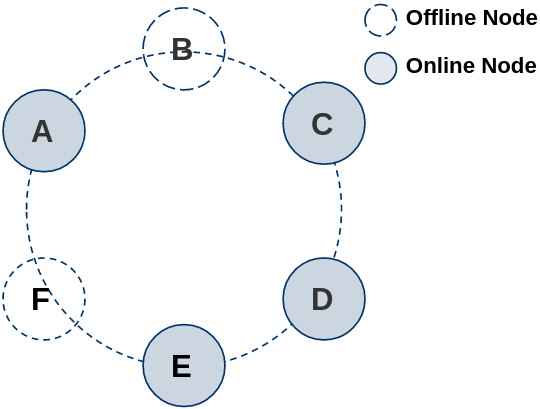
\includegraphics[width=0.4\textwidth]{assets/dht.png}
    \caption{DHT nodes arranged by ID in a circular list. The data for a node is persisted by the two subsequent online nodes. In this example the messages for A and B are both persisted by C and D}
    \label{fig:dht}
\end{figure}

What peers serve as backup-peers for another peer obviously changes when new peers connect to the network or go offline.
Consider the setup shown in figure \ref{fig:dht}, where node C and D are the backup-peers for both, A and B. 
If now C would suddenly go offline, there would be only one back-up peer left, that may go offline at some point themselves. 
We solved this by having nodes dynamically re-publish storage message when peers connect / disconnect. 
Concretely this means that if node C would go offline, node D would be informed of this and notice (by referring to the shared list of sorted online peers) that C was backup for A and B. 
As the second back-up node, D stores the same data and thus can send it to the next online node in the list, node E.
D and E would then be the two new backup peers for A and B.
For the messages of node C no new storage is necessary because D and E are already backing its data up. 
Similar when a new node comes online it becomes a back-up node for all nodes up until the next two preceding online nodes.
Another node that was previously backing up the data is not required to do it anymore. 
It sends the data to the new peer for storage and clears it from its own memory.
For instance in figure \ref{fig:dht} if node B would join the network again, it becomes a backup node for A, F and E. 
D would now not be a backup for A anymore and C would not be one for E and F anymore. 
C and D would both send the data of those nodes to B and themselves stop storing it.



